\section{Three paths force a large shadow}\label{sec:shadow}

Put $b=0.43892$. We use a straight unit segment, a planar polygonal arc
of minimum planar width greater than $b$, and a particular polygonal arc
$G$ in three dimensions. Each path can have its own rigid placement.
Throughout this section, area means two-dimensional Lebesgue measure.

\paragraph{Projection along the unit segment.}
Let $u$ be the direction of the segment in a universal body $K$ and
let $P$ be the orthogonal projection of $K$ onto $u^\perp$. The plane of
the placed planar arc contains a direction perpendicular to $u$. Projection
preserves its width in that direction, so $P$ has diameter greater than
$b$ and contains a straight chord of length $b$. Rotate horizontal
coordinates to make this chord parallel to the $x$-axis.

Write $\ell(y)$ for the length of the fiber of $K$ over $y\in P$.
The fiber over the projected unit segment $y_0$ has length at least one.
Joining both endpoints of that segment to one point over each $y$ gives
$\ell(ty_0+(1-t)y)\ge t$. Thus
\[
 |K|=\int_P\ell(y)\,dy
 \ge |P|\int_0^1(1-t)^2\,dt=\frac{|P|}{3}.
 \tag{1}\label{eq:fiber}
\]
Up to a translation, $P$ also contains an orthogonal projection of a
rotation of $G$. A translation of the whole picture lets us fix that
projection at the origin of our coordinate system and let the chord
translate freely. We will prove that every such planar convex set
has area greater than $0.05826$.

\paragraph{The two polygonal witnesses.}
The planar path's $69$ vertices are specified by the integer table and
reflection in \texttt{lower/check\_planar.py}. They sample the planar
caliper of Adhikari and Pitman \cite{caliper}. Divide the coordinates by
$2{,}278{,}289{,}034$, the sum of $1+\lfloor\sqrt{m}\rfloor$ over the
squared integer link lengths $m$. Its length is less than one. To bound its
width from below, test the normals to the differences of each of the $2346$
pairs of points. Between consecutive directions at which projections of
two vertices tie, the extreme vertices are fixed and the width $f(\theta)$
satisfies $f''=-f<0$. Its minimum is therefore at a tested endpoint.
For every pair the code squares and compares the integer projection span
with $b$ times the length of its normal, accounting for the denominator.
All tests are strict. This verifies the needed width directly.

The successive $61$ vertices of the spatial arc $G$ are the integer
triples in \texttt{lower/witness.hpp}, in units of $10^{-7}$. We obtained
them by deforming the inspection polygon of the linked refinement
\cite{refinement} to increase the area forced by its projections and the
chord. Their displayed integer coordinates are the definition of $G$.
Writing $F=\operatorname{conv}G$ and $B_3$ for the unit ball, the exact
checks give
\[
 L(G)<0.9999830,\qquad 0.102 B_3\subseteq F\subseteq 0.245 B_3 .
 \tag{2}\label{eq:balls}
\]
The length check uses the same integer square-root bound as above.
Checking the outer radius only needs squared vertex norms. Four affinely
independent vertices certify full dimension. Every facet plane of $F$
passes through a noncollinear triple, so enumerate all such triples.
If all vertices are on one side, choose the outward normal $n$ and
offset $s$. In the integer coordinates the program checks $s>0$ and
$s^2\ge 1{,}020{,}000^2\|n\|^2$ for each of the $118$ supporting
triples. Intersecting the facet half-spaces proves the inball claim.
The included script \texttt{lower/check\_witness.py} carries out these tests.
Shorter curves are legitimate by the closure argument in Section~\ref{sec:setting}.

\section{An area test with the chord free to move}\label{sec:planar}

For a compact convex set $D$ and vector $n$, write
$h_D(n)=\max_{v\in D}n\cdot v$. Given finitely many planar points known
to lie in the shadow, the following test bounds the area uniformly in the
position of the horizontal chord.

\noindent\begin{minipage}{\linewidth}
\centering
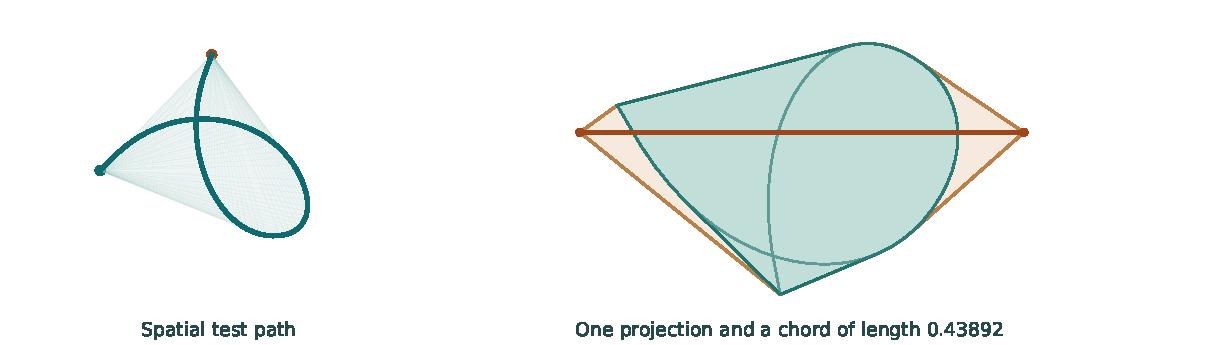
\includegraphics[width=.83\linewidth]{lower/shadow.pdf}\par
\raggedright\small
The planar picture shows one orthogonal shadow of the spatial witness and
one position of the compulsory chord. The orange boundary is their joint
convex hull. The proof allows every rotation of the path and every
translation of the chord.
\end{minipage}

\paragraph{Centering horizontal slices.}
Replace the intersection of a convex set with each horizontal line by an
interval of the same length centered on the $y$-axis. The result is
convex, because the interval length is a concave function of height:
interpolating two intervals gives a subinterval of the corresponding
intermediate slice. Fubini's theorem gives equality of areas, and inclusion
of sets is preserved. In particular the symmetrized shadow still contains
a chord of length $b$, now centered at $(0,c)$ for some unknown real $c$.

Let $Q$ be any polygon contained in the symmetrization of the known points'
convex hull. In the verifier all lengths at this stage are in units of
$10^{-6}$, so the chord length is the integer $d=438920$. Orient the
vertices $v_i$ of $Q$ counterclockwise. For an edge vector
$(\Delta x_i,\Delta y_i)$ put $n_i=(\Delta y_i,-\Delta x_i)$ and
$o_i=n_i\cdot v_i$. If a planar body $D$ contains $Q$ and a horizontal
segment of length $d$ centered at $(0,c)$, then
\[
 2|D|\ \ge\ 2|Q|+\sum_i
 \left[\frac{d}{2}|n_{ix}|+c\,n_{iy}-o_i\right]_+,
 \qquad [a]_+=\max(0,a).                         \tag{3}\label{eq:mix}
\]

\emph{Proof.} Let $M$ be the hull of $Q$ and the segment. For any two
convex polygons $Q,M$, the coefficient of $t$ in $|Q+tM|$ is
$\sum_i h_M(n_i)$. To see this, translate $M$ to contain zero. At
first order each edge sweeps a strip of length $\|n_i\|$ and width
$t h_M(n_i)/\|n_i\|$; the finitely many corner contributions have
area $O(t^2)$. Translation does not affect the sum since $\sum_i n_i=0$.
The edge list of $Q+tM$ is formed by merging the cyclic edge lists
of $Q$ and $tM$, since the face exposed by each normal is the sum of
the two exposed faces. Its starting vertex is likewise a sum. The
shoelace formula therefore makes $|Q+tM|$ a quadratic in $t$.
Its constant coefficient is $|Q|$, and its leading coefficient is
$|M|$ by rescaling and taking $t\to\infty$. Since $Q\subseteq M$,
we have $Q+tM\subseteq(1+t)M$. Cancelling the quadratic terms,
dividing by $t$ and letting $t\to\infty$ bounds the linear coefficient
by $2|M|$. Now $h_M(n_i)=\max(o_i,d|n_{ix}|/2+c n_{iy})$ and
$\sum_i o_i=2|Q|$. As $M\subseteq D$, this proves \eqref{eq:mix}.
\hfill$\square$

\paragraph{One-variable minimization.}
The right side of \eqref{eq:mix} is a convex piecewise-linear function
of $c$. On scaling the sum by two, its individual terms are
$[a_i+b_i c]_+$, where $a_i=d|n_{ix}|-2o_i$ and $b_i=2n_{iy}$.
The initial slope is $\sum_{b_i<0} b_i$ and each finite breakpoint
$-a_i/b_i$ contributes an upward jump of $|b_i|$. Sorting the rational
breakpoints and taking the first at which the accumulated slope is
nonnegative gives the global minimum, including a flat interval of
minimizers. Terms with $b_i=0$ are simply constants. Thus the test
eliminates every possible chord translation by integer comparisons.

For integer input points, compute the left and right boundary chains of
their hull in order of increasing height. At every vertex height
interpolate both endpoints of the horizontal slice and round its
half-length down to an integer. Take the hull of the resulting pairs of
opposite slice endpoints to form $Q$. Each pair is in the centered
slice, so all these inward roundings preserve \eqref{eq:mix}. The chain
algorithm discards the middle of any successive triple that bends in the wrong direction for the required chain. The lower convex and upper concave envelopes in coordinates $(y,x)$ thus give the two slice endpoints. Even omitting interior heights would only shrink the polygon used for the lower bound.

\section{A finite proof for every rotation}\label{sec:rotation}

We describe the coverage of the rotation group and the error estimate
explicitly. The only inputs to the loop are the integer vertices, the
chord length, the bounds in \eqref{eq:balls}, and the claimed area
threshold. There is no stored list of successful rotations.

Identify a rotation with quaternion conjugation by a nonzero
quaternion $q=(q_0,q_1,q_2,q_3)$, normalized by $\|q\|^2$.
Every proper rotation has such a representation: a rotation of angle
$\theta$ about a unit axis $u$ is represented by
$\cos(\theta/2)+u\sin(\theta/2)$. Left multiplication by one of
$1,i,j,k$ can move a component of largest magnitude into the scalar
position. On rotated vectors this just applies a coordinate half-turn,
so the projected figure changes at most by signs of its two coordinates.
Area and the constraint on a horizontal unoriented chord are preserved.
Rescale the quaternion to put its scalar component equal to $1$.
It suffices to check the single parameter cube $(q_1,q_2,q_3)\in[-1,1]^3$.

\paragraph{A polygon valid on an entire cell.}
At subdivision depth $k$ put $m=2^k$. In homogeneous integer coordinates
the center quaternion is $q=(m,v_1,v_2,v_3)$, with each free coordinate
of any other quaternion $q'$ in the cell differing by at most one.
Let $L$ be the floor of
\[
 \sqrt{m^2+\sum_{j=1}^3 \max(0,|v_j|-1)^2}.
\]
Both quaternion lengths are at least $L$. Their unit representatives
differ by at most $\sqrt3/L$. Indeed for nonzero $a,b$,
\[
 \|a-b\|^2=(\|a\|-\|b\|)^2+
  \|a\|\|b\|\left\|a/\|a\|-b/\|b\|\right\|^2 .
\]
For unit quaternions $s,t$, write $s x\bar s-t x\bar t$ as
$(s-t)x\bar s+t x(\bar s-\bar t)$. Its norm is at most
$2\|s-t\|\|x\|$. Thus, in units of $10^{-6}$, every projected vertex
moves by at most
\[
 \varepsilon=\lceil849000/L\rceil,
 \qquad 2\sqrt3\,245000<849000.
\]
If the center's vertical projection span, less $2\varepsilon$, is $s$,
then the true transverse span is at least $s$. Taking triangles on the
horizontal chord from the two transverse extremes of the entire planar
container gives twice-area at least $ds$. The chord lies between those
extremes and the two triangle interiors are disjoint. This yields a
quick test when $ds$ exceeds the threshold. Otherwise form a common
inner polygon as follows.

Write $B_0$ for the projected hull at the center and $B$ for the true
projected hull at any parameter in the cell. For every unit planar $n$,
$h_{B_0}(n)\le h_B(n)+\varepsilon$ and $h_B(n)\ge r=102000$ in
these units. Scale every center projection by
$\alpha=(r-2)/(r+\varepsilon)$ and truncate both coordinates towards
zero to integers. Each rounding error has norm less than $2$. For the
hull $J$ of the resulting points,
\[
 h_J(n)\le \alpha(h_B(n)+\varepsilon)+2\le h_B(n).
\]
The last inequality follows by substituting $h_B(n)\ge r$. A point outside a compact convex set is strictly separated by the line through its nearest point perpendicular to the joining segment. The support inequalities thus give $J\subseteq B$ throughout the cell.
The area test of Section~\ref{sec:planar} can therefore use $J$.

\paragraph{Exhaustion and exact arithmetic.}
Start at $(m,v)=(1,0)$. If neither the span nor the polygon test proves
the claimed strict inequality, replace the cell by its eight children
$(2m,2v+\sigma)$ for $\sigma\in\{-1,1\}^3$. The closed children
cover their parent. The implementation computes the center rotation with
the integer quadratic quaternion matrix, keeping the common denominator
until the rounding just described. All geometric decisions and
breakpoint comparisons are exact. The verifier treats a depth-limit
failure as an unresolved proof. The C++ implementation uses signed 64-bit coordinates and signed 128-bit products. At its depth limit $16$ the squared quaternion norm is at most $4\cdot 2^{32}$. A matrix row has Euclidean length equal to this norm, so each intermediate three-term dot product stays below $3\cdot 4\cdot 2^{32}\cdot2{,}450{,}000<2^{57}$. The scaled and rounded planar coordinates have magnitude below $245001$; the products used to compare rational breakpoints or polynomial areas are formed in 128 bits. The run visits $35{,}533{,}409$ cells, terminating $739{,}854$ by span
and $30{,}351{,}879$ by polygon area. The remaining $4{,}441{,}676$
are split, with greatest depth $14$. In particular, no unresolved terminal
cell is counted. Successful exhaustion gives
\[
        2|P|>116520000000\cdot10^{-12}=0.11652.
\]
The area factor in \eqref{eq:fiber} then proves $|K|>0.01942$.
The minimum is attained by Section~\ref{sec:setting}, so its lower bound
is strict as well.
